\section{Intrinsic filtering for 2D manifold surface}

In this section, we introduce our intrinsic filtering model for 2D manifold surfaces in detail.
Furthermore, we explain that almost all classical filtering methods can be viewed as a simplification of ours.

\subsection{Filtering for 2D manifold surface}

Suppose we are interested in signals that are defined on 2D manifold surface $\Omega$ with values in domain $\Gamma$,
the filtered output signal $\bar{J_p}$ at point $p$ can be produced by this general form
\begin{equation}
\label{Eq:GeneralForm}
\bar{J_{p}} = \frac{1}{W_{p}}\int_{\mathcal{N}(p)}\omega_{p, q}J_{q}d_{q}\, ,
\end{equation}
where $J_{q}$ denotes the value of the signal at point $q$; $\mathcal{N}(p)$ is the neighborhood of the point $p$;
$\omega_{p, q}$ indicates the weight for each neighboring signal,
and $W_{p} = \int_{\mathcal{N}(p)}\omega_{p, q}d_{q}$ is the normalization factor for ensuring the sum of all $\omega_{p,q}$ equal to 1.
The construction of $\omega_{p,q}$ is very important, it directly relates to the performance of edge-preserving.

Here, we give the following weight which reflects the cumulative difference of input signal:
\begin{equation}
\label{Eq:IntrinsicWeight}
\omega_{p,q} = g(d^{s}(\varphi_{p}, \varphi_{q}); \sigma_{s})g(d^{r}(\psi_p, \psi_q); \sigma_{r})\, ,
\end{equation}
where we choose Gaussian function as kernel function $g(\cdot \,; \cdot)$, $\sigma_{s}$, $\sigma_{r}$ are variance parameters and the function $d^s$ and $d^r$ are defined as:
 \begin{equation}
 \label{Eq:IntrinsicDistance}
 \left \{
 \begin{array}{ll}
        d^{s}(\varphi_p, \varphi_q) = \lim_{\Delta{s}\to 0} (\int_{L}||\varphi_{q_{s + \Delta{s}}} - \varphi_{q_s}||^{n}ds\,\,)^{1/n} \vspace{1.5mm} \\
        d^{r}(\psi_p, \psi_q) = (\int_{L}||\psi_{s} - \psi_{p}||^{m}ds\,\,)^{1/m} \\
 \end{array}
 \right. .
 \end{equation}

Note that $L$ is the geodesic path connecting points $p$ and $q$.
$\varphi$ and $\psi$ can represent different signals, for example position, Gaussian curvature and normal on a 2D manifold surface.
$q_{s + \Delta{s}}$, $q_s$ and $s$ are points in path $L$.

The cumulative difference of input signal can reflect the local structure of desired signal.
The main reason is that we consider the difference not only between adjacent signals but also start-end signals.
According to different problems, we can choose suitable parameters $\varphi$, $\psi$, $n$ and $m$.

Equation \ref{Eq:IntrinsicDistance} which reflects the similar differences between signals can be approximated as:
 \begin{equation}
 \label{Eq:IntrinsicDiscreteDist}
 \left \{
 \begin{array}{ll}
        d^{s}(\varphi_p, \varphi_q) = (\sum_{q_{i+1}, q_i \in{L}}|\!|\varphi_{q_{i+1}} - \varphi_{q_i}|\!|^{n}|\!|q_{i+1} - q_{i}|\!|\,)^{1/n} \vspace{1.5mm}\\
        d^{r}(\psi_p, \psi_q) = (\sum_{q_{i+1}, q_i \in{L}}|\!|\psi_{q_i} - \psi_{p}|\!|^{m}|\!|q_{i+1} - q_{i}|\!|\,)^{1/m}
 \end{array}
 \right. .
 \end{equation}
We define $|\!|q_{i+1} - q_{i}|\!|$ as a step length in the above formula.
As image is a special 2D manifold, some classical filtering methods~\cite{tomasi1998bilateral, grazzini2009edge, Chang2015propagated} are special cases of our method.
We think about the 4-neighbor connecting in image, so the step length is $||q_{i+1} - q_{i}|| = 1$ in image filter. %a geodesic path $L$.
Next, we explain why our method are generalized.

{\bfseries Case 1.}
Bilateral filter~\cite{tomasi1998bilateral}, as a classical nonlinear filter, uses two Gaussian functions as the spatial and range weights respectively.
In our generalized model~\ref{Eq:IntrinsicDiscreteDist}, we use two points $p$ and $q$ to replace the geodesic path $L$.
At the same time, signal functions $\varphi$ and $\psi$ are defined as $\varphi_{x} = x$ and $\psi_{x} = I_x$,
where $x$ is the pixel position and $I_x$ respectives the pixel intensity.
When $m=2$ and $n=2$, our model is simplified as:
\begin{equation}
\label{Eq:BilateralDistance}
\left \{
\begin{array}{ll}
        d^{s}(p, q) = ||p - q|| \vspace{1.5mm}\\
        d^{r}(I_{p}, I_{q}) = || I_{p} - I_{q} || \\
\end{array}
\right. .
\end{equation}
We can see that the above formulation gets the distance differences, which are used to calculate the weights in bilateral filtering.

{\bfseries Case 2.}
Geodesic filtering~\cite{grazzini2009edge} only uses accumulative difference in adjacent pixel signals during filtering process.
This way gives a high response in image edges, so has a better edge-preserving power than bilateral filtering.
Namely, when $n=2$, the image intensity value $I$ as a signal value $\varphi$ and $d^{r}(\psi_p, \psi_q) = 1$,
our intrinsic filtering is simplified, gets the distance difference between intensities of geodesic image filtering:
 \begin{equation}
 \label{Eq:GeodesicDistance}
 \left \{
 \begin{array}{ll}
        d^{s}(I_p,I_q) = (\sum_{q_{i+1}, q_i \in{L}}||I_{q_{i+1}} - I_{q_i}||^{2}\,)^{1/2} \vspace{1.5mm} \\
        d^{r}(\psi_p, \psi_q) = 1 \\
 \end{array}
 \right. .
 \end{equation}

{\bfseries Case 3.}
In a similar way, our intrinsic filtering is simplified as a propagation image filtering~\cite{Chang2015propagated} by $n=2$, $m=2$, $\varphi$ and $\psi$ both represent the pixel intensity.
Therefore,
 \begin{equation}
 \label{Eq:PropagationDistance}
 \left \{
 \begin{array}{ll}
        d^{s}(I_p, I_q) = (\sum_{q_{i+1}, q_i \in{L}}||I_{q_{i+1}} - I_{q_i}||^{2}\,)^{1/2} \vspace{1.5mm}\\
        d^{r}(I_p, I_q) = (\sum_{{q_i} \in{L}})||I_{q_i} - I_p||^2\,)^{1/2} \\
 \end{array}
 \right. .
 \end{equation}
It is more comprehensive in considering the difference between signals.
It has an outstanding power in preserving the image edge structures.


\begin{figure}
\centering
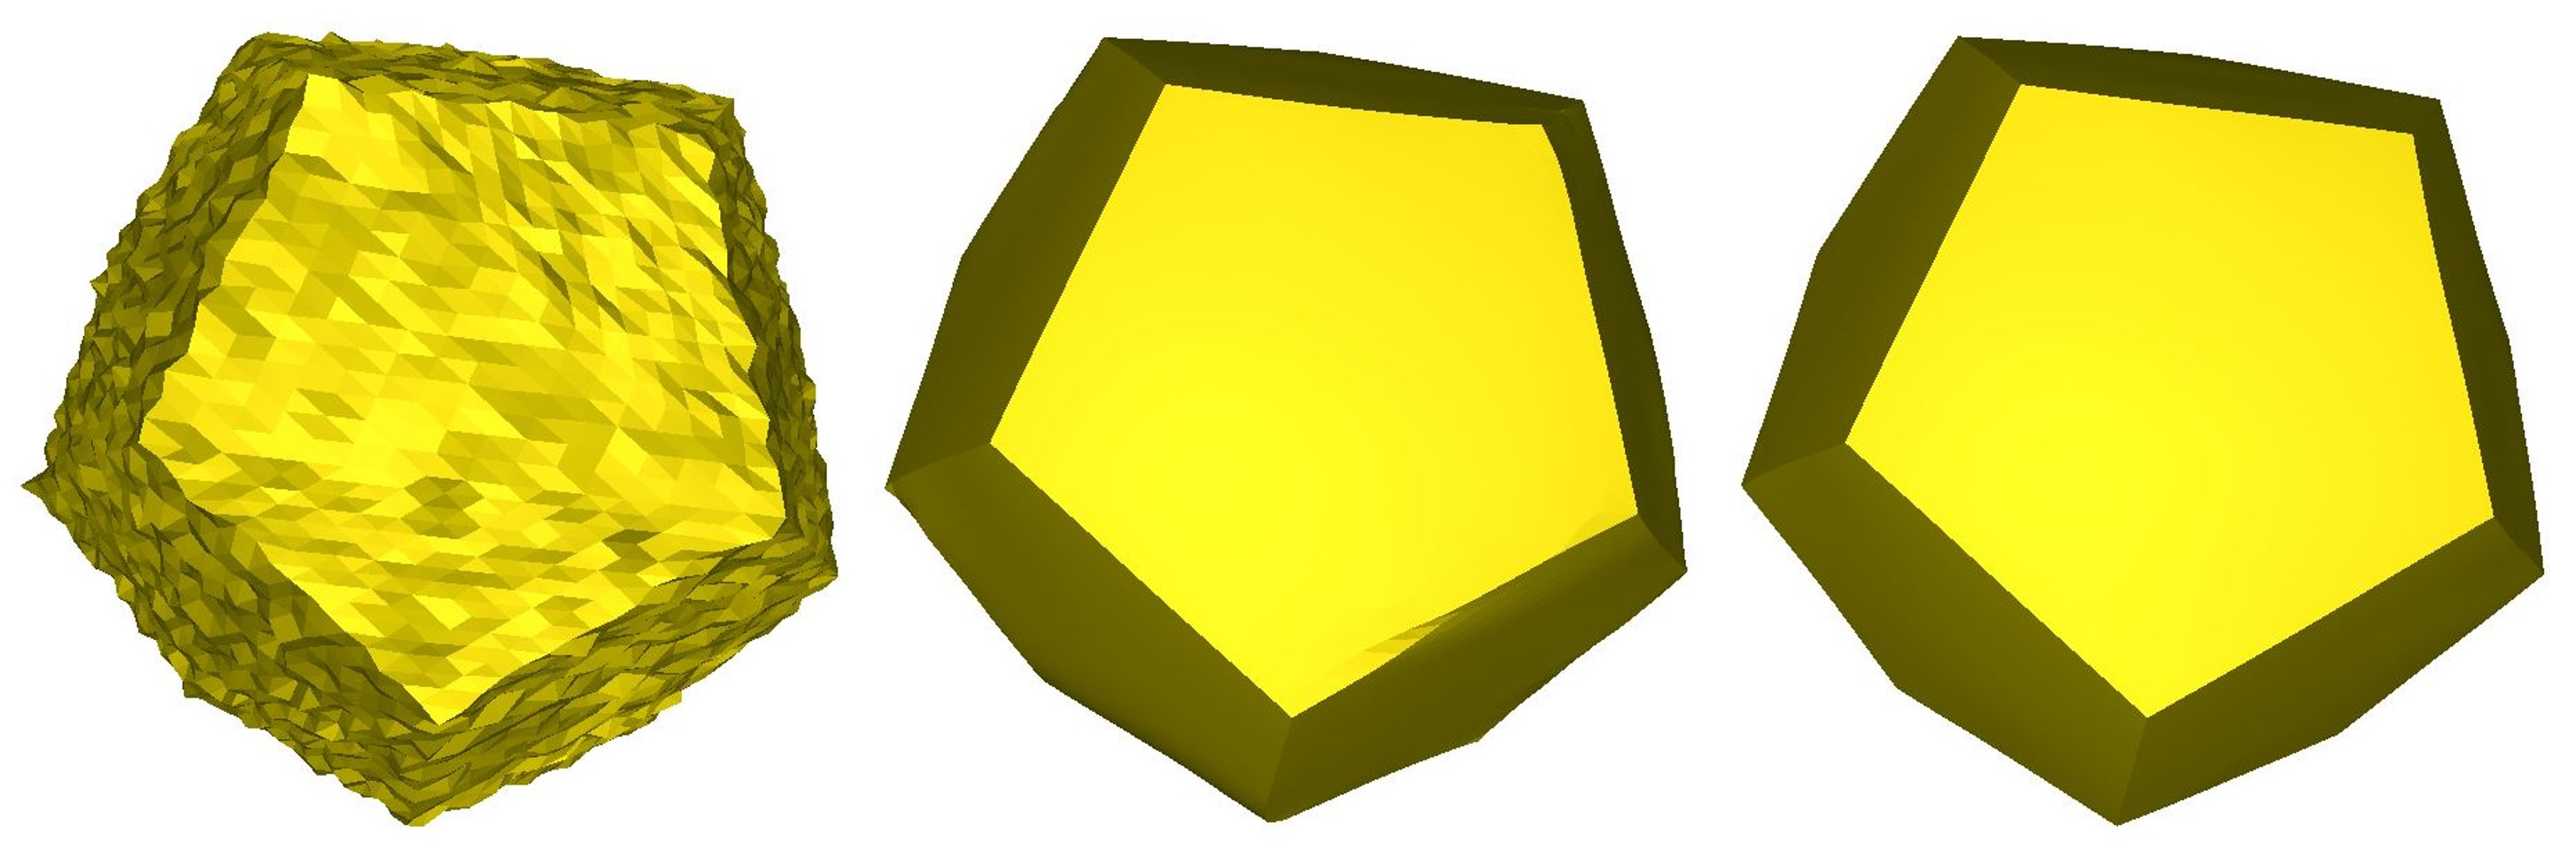
\includegraphics[width = 7.0cm]{results/shortest/shortest.jpg}
\vspace{-0.5mm}
\caption{ Comparison between geodesic paths and square-pattern paths. Left: the noisy mesh selected from~\cite{Wang2014decoupling}. Middle: the result of applying geodesic paths. Right: the result of applying square-pattern paths. The parameters of these two strategies are the same ($k_{iter} = 30$, $v_{iter} = 2$, $r = 4$, $\sigma_r = 0.3$ ). The time consumption is about 22.76s and 2.55s respectively. The former is not good in dealing with straight edges.}
\label{Fig:shortestpath}
\end{figure}

Our intrinsic filtering builds connections between $p$ and $q$, which providing more reliable information about the structure of the desired output.
This relation can be depicted in Figure \ref{Fig:relation}.
Our method inherits the advantage of these filtering algorithms~\cite{tomasi1998bilateral, grazzini2009edge, Chang2015propagated} while compensating their deficiencies,
and becomes more adaptive to the context of input signals.


\subsection{Filtering mesh geometry}

Given a noisy triangle mesh, our goal is to filter the noise while keeping the mesh structure.
In order to achieve this purpose, we adapt a two-stage process which be widely used in mesh filtering.
Firstly, noisy face normals are filtered iteratively by our intrinsic filtering model. %by equation~\ref{Eq:IntrinsicMeshFiltering}.
Secondly, according to the filtered face normals, vertex positions are updated iteratively though gradient descent.

{\bfseries Filtering face normals.}
When we consider normals as a surface signal defined over the original triangle mesh, it is easy to put the intrinsic filtering algorithm to mesh denoising.
For a triangle face $f_{i}$, its outward normal $\mathbf{n_{i}}$ can be calculated by outer product easily.
Then we consider $\mathbf{n_{i}}$ as a signal associated with the face centroid $c_{i}$.
In order to filter the face normals $\mathbf{n_{i}}$, we need find a path $L$ to connect $\mathbf{n_{i}}$ and its neighbor $\mathbf{n_{j}}$.
Finally, a filtered face normal $\bar{\mathbf{n_{i}}}$ is computed through our intrinsic mesh filtering model:
 \begin{equation}
 \label{Eq:IntrinsicMeshFiltering}
 \bar{\mathbf{n_{i}}} = \frac{1}{W_{i}}\sum_{\mathclap{f_{j}\in\mathcal{N}_{i}}}A_{j}g(d^{s}(\mathbf{n_{i}}, \mathbf{n_{j}}); \sigma_{s})g(d^{r}(\mathbf{n_{i}}, \mathbf{n_{j}}); \sigma_{r})\mathbf{n_{j}}\, .
 \end{equation}
  here,
 \begin{equation}
 \label{eq:IntrinsicMeshDistance}
 \left \{
 \begin{array}{ll}
        d^{s}(\mathbf{n_{i}}, \mathbf{n_{j}}) = (\sum_{x, x+1\in{L}}||\mathbf{n_{x+1}}-\mathbf{n_{x}}||^{n}\,\,)^{1/n} \vspace{1.5mm} \\
        d^{r}(\mathbf{n_{i}}, \mathbf{n_{j}}) = (\sum_{x\in{L}}||\mathbf{n_{x}}-\mathbf{n_{i}}||^{m}\,\,)^{1/m} \\
 \end{array}
 \right. ,
 \end{equation}
where $W_{i}$ is the normalization factor,
calculated by
$||\sum\limits_{\mathclap{f_{j}\in\mathcal{N}_{i}}}A_{j}g(d^{a}(\mathbf{n_{i}}, \mathbf{n_{j}}); \sigma_{s})g(d^{r}(\mathbf{n_{i}}, \mathbf{n_{j}}); \sigma_{r})||$
which ensures that $\bar{\mathbf{n_{i}}}$ is a unit normal;
$A_j$ is the area of face $f_j$;
$\mathcal{N}_{i}$ is the neighborhood of face $f_{i}$.
In our paper, we use the geometrical neighborhood, defined at the paper~\cite{Zhang2015Filter}.

Note that equation \ref{Eq:IntrinsicMeshFiltering} can be derived from equation \ref{Eq:GeneralForm}.
$A_j$ is the accumulation of infinitesimal area because the domain of integration is triangle face.
Furthermore, we give up the step length which measures the distance between adjacent centroid of triangle faces. % to facilitate the calculation in equation \ref{eq:IntrinsicMeshDistance}.
We simply make this term be one for facilitating the calculation.

Although the geodesic algorithm gives the shortest distance $d^s$ and $d^r$, it is computationally expensive.
Considering the shortcomings, we introduce a simple, fast and effective pattern for choosing filtering paths which is shown in next section.
We find that this operation is about an order of magnitude faster than applying shortest path in obtaining similar results.
Furthermore, the filter results that applying the particular paths often are more powerful on dealing with details, like edges and corners.
These results are shown in the figure \ref{Fig:shortestpath}.

\begin{figure}%[htb]
\centering
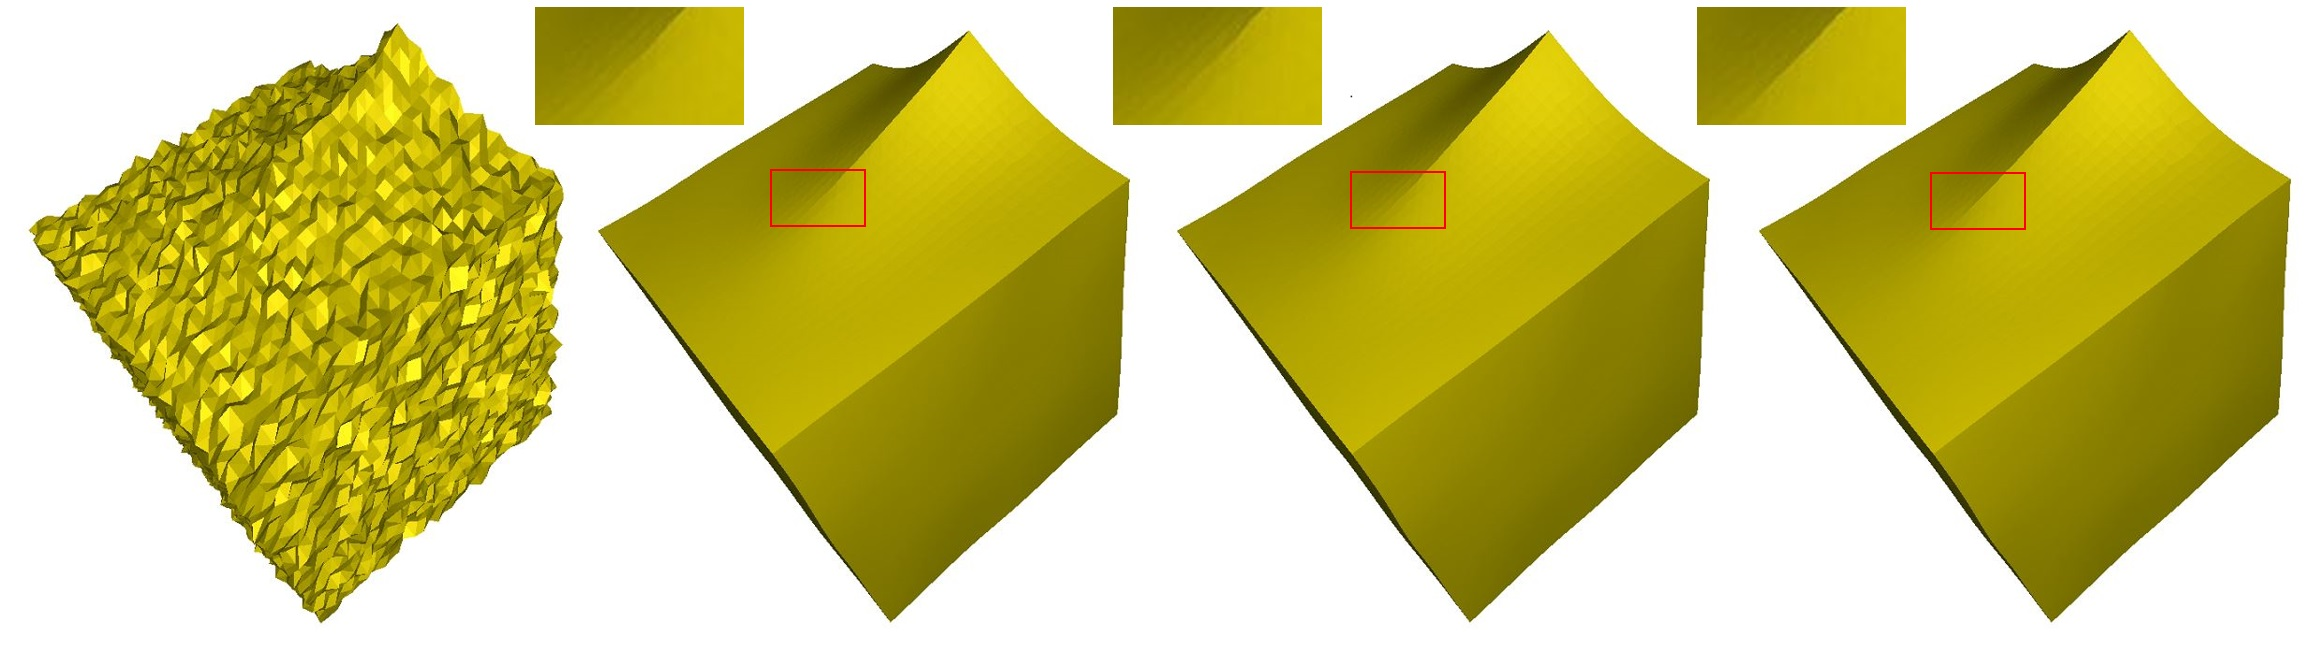
\includegraphics[width = 7.5cm]{results/Norm/norm.jpg}
\vspace{0.5mm}
\caption{ From the left to right: Noised mesh ( Gaussian noise with 0.3$\sigma_E$ ), the results of $m = n = 2$ with step length,
$m = n = 2$ without step length, $m = n = 1$ without step length.
Because of the sparseness of mesh feature, $L_1$ norm receives the best results in preserving the mesh structure.}
\label{Fig:norm}
\end{figure}

\begin{figure}
\centering
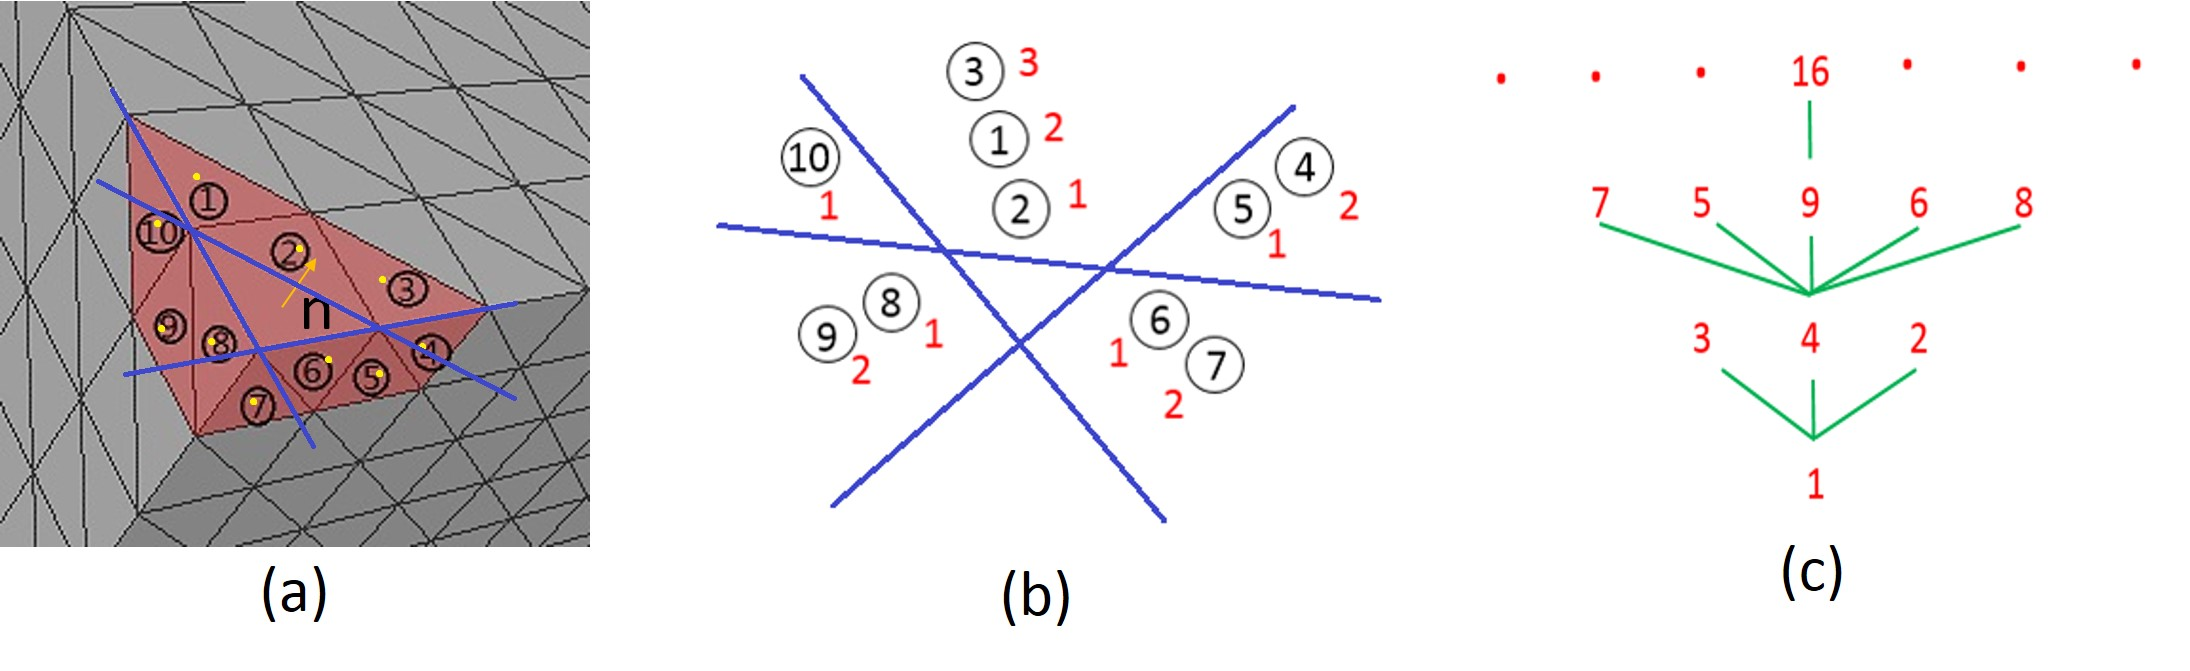
\includegraphics[width = 7.5cm]{results/Path/path1.jpg}
\vspace{-3mm}
\caption{ The process of generation path. (a) the 10 neighbors of current face with its normal $\mathbf{n}$. (b) The schematic diagram after projection, dividing and sorting. (c) the pattern.
The numbers with circle are the neighbor of current triangle face, the yellow points are the projection points of neighbor face centroid, the blue lines are used to decide the face label, the red numbers are their serial number after sorting, the green lines are connected path.}
\label{Fig:path}
\end{figure}

For triangle mesh, we conduct the experiment in the presence of $m$ and $n$ taking different values.
We mainly implement three group experiments. Figure~\ref{Fig:norm} show the denoised results of different conditions.
We find that $m=1$ and $n=1$ can obtain the best results because of the sparseness of mesh feature.
From the figure~\ref{Fig:norm}, the $L_1$ norm is more sensitive to details, so has a better expression.

 {\bfseries Updating vertices.} After all face normals is filtered, the vertex positions need to be updated to cater to these new normals.
 We adopt the iterative scheme in the paper~\cite{sun2007fast} to update the vertex positions.
 Namely, for a face $f_{i}$, we calculate its updated vertex positions via the following iteration form
 \begin{equation}
 \label{vertexupdate}
 \bar{v_{i}}^{(t+1)} = \bar{v_{i}}^{(t)} + \frac{1}{|{\mathcal{F}_{i}}|}\sum_{j\in\mathcal{F}_{i}}\mathbf{\bar{n}_{j}}[\mathbf{\bar{n}_{j}}\cdot(\bar{c_{j}}^{(t)}-\bar{v_{j}}^{(t)})]\, ,
 \end{equation}
 where $\bar{v_{j}}^{(t)}$ is the value of $\bar{v_{i}}$ in the $t-th$ iteration,
 $\mathcal{F}_{i}$ is the index set of the incident faces for $\bar{v_{i}}$,
 $|\cdot|$ denotes the cardinality of a set,
 and $\bar{c_{j}}^{(t)} = \sum_{i=1}^{3}\bar{v_{j_{i}}}^{(t)}/3$ is the centroid of the triangle $f_{j}$.
 This scheme is actually based on the orthogonality between the normal and the three edges of each face on the mesh.
 Then adopts a gradient descend process for solving that orthogonality equation in the conditions of  $L_2$ error.

 In our experiments, 10 to 20 iterations are sufficient for achieving satisfactory results and approximately up to above conditions.
 Our filtered process is summarized in Algorithm~\ref{alg:1}.
 In the next section, we introduce a simple but effective method for selecting a particular pattern for our propagated mesh filtering.



\begin{algorithm}\caption{Intrinsic mesh filtering framework}
\label{alg:1}
\begin{algorithmic}
\STATE {\textbf{Input:} Initial mesh $M_{in}$, number of iterations $k_{iter}$.}
\STATE{\textbf{Output:} Filtered mesh $M_{out}$.}
\STATE{1: $M^{(0)} = M_{in}$}
\STATE{2: Compute the path sets $\mathcal{N}$} according to section \ref{Sec:path}.
\STATE{3: \textbf{for} $s = 1$ to $k_{iter}$ \textbf{do}}
\STATE{4: ~~~Compute face normals {$n_i$} of mesh $M^{(s-1)}$;}
\STATE{5: ~~~Get paths from {$\mathcal{N}_i$} to {$n_i$};}
\STATE{6: ~~~Compute filtered normals {$\mathbf{\bar{n_i}}$} according to~\ref{Eq:IntrinsicMeshFiltering};}
\STATE{7: ~~~Compute updated mesh $M^{(s)}$ according to {$\mathbf{\bar{n_i}}$};}
\STATE{8: \textbf{end for}}
\STATE{9: $M_{out} = M^{k_{iter}}$.}
\end{algorithmic}
\end{algorithm}



 \section{Path chosen for mesh filtering}
 \label{Sec:path}



 In image, many particular patterns can be chosen because of the regular coordination system.
 These patterns are simple and easy to be thought about.
 But in triangle mesh, it is very difficult to obtain a good pattern which can preserve the mesh feature.
 The easiest way to be thought of is applying the shortest path algorithm on the triangle mesh.
 However, figure \ref{Fig:shortestpath} shows this method is time consuming.
 We solve this problem in this paper within the context of mesh denoising.

 Our method is based on the following theory: the areal coordinates of triangle segments the plane into seven regions.
 Areal coordinates are extremely useful in engineering applications involving triangular subdomains.
 These make analytic integrals often easier to evaluate, and Gaussian quadrature tables are often presented in terms of area coordinates.
 In the context of a triangle, the areal coordinates of a point $P$ are the ratios of the areas of $PBC$, $PCA$ and $PAB$ to the area of the reference triangle $ABC$.
 %shown in the figure~\ref{Fig:path}(a).
 Because the ratios are a plus or a minus, it divide the plane where the triangle is to seven parts.
 That gives us an enlightenment to obtain a particular pattern for solving the problem of paths.

{\bfseries Path generation.}
For each triangle $f_i$, we project its neighborhood $\mathcal{N}_i$ onto a tangent plane basing its normal $\mathbf{\bar{n_i}}$.
In detail, we only project their centroid onto that plane.
Then basing the three points of $f_i$, we use areal coordinations to divide these centroid to seven regions.
Note that, if the projection point falls into the face $f_i$, we throw it away from $\mathcal{N}_i$.
In this way, we give each neighbor a label that belong to a specified region.
Afterwards, we sort these neighbors belong to the same region according to their face centroid distance to $c_i$ in original noisy mesh.
Finally, we provide a particular pattern to assign the path for matching the ordered neighbors.
This pattern is defined square-pattern, which is used for generating paths.
The entire process is depicted in the figure~\ref{Fig:path}.

{\bfseries Advantages.}
 The above process has the power to protect local mesh feature like edge and corner.
 To a certain extend, the six regions surrounding $f_i$ depict the local structure of a mesh.
 Projecting along the normal of $f_i$ makes the faces having similar normal flock together.
 Furthermore, the division further restricts the normal difference according to areal coordinates.
 The combination of these two aspects insures that one of six regions has the similarity to $f_i$.
 The part including faces $\textcircled{1}$, $\textcircled{2}$ and $\textcircled{3}$ has the similar normal to $f_i$ in the figure \ref{Fig:path}(b).
 These normals play a important role in applying our intrinsic filtering algorithm.

 Figure \ref{Fig:path}(c) shows the square-pattern for generating path.
 We use $n^2$($ n = 1, 2,...$) as connection points, the sequence numbers between $(m-1)^2$ and $m^2$ including $m^2$ directly connect the number $(m-1)^2$.
 In this way, paths are generated.
 For example, the path between number $8$ and $f_i$ is $8-4-1-f_i$, number $16$ and $f_i$ is $16-9-4-1-f_i$ and so on.
 Once generating the paths, they will not change in the subsequent iterations.

 In the next section, we will introduce the experimental results basing our method.
